% ---------------------------------------------------------------------------
% Lab 1 - AI and Cybersecurity
% Compile with pdfLaTeX on Overleaf (no bibliography, no external packages
% beyond the standard TeX Live ones).
%
% Structure:  main.tex  +  figures/*.png
% ---------------------------------------------------------------------------
\documentclass[9pt]{extarticle}

\usepackage[T1]{fontenc}
\usepackage[utf8]{inputenc}
\usepackage{newtxtext,newtxmath}      % Times-like font, as in the template
\usepackage[a4paper,margin=1in]{geometry}
\usepackage{graphicx}
\usepackage{booktabs}
\usepackage{longtable}
\usepackage{array}
\usepackage{amsmath}
\usepackage{microtype}
\usepackage{enumitem}
\usepackage{caption}
\usepackage{titlesec}
\usepackage[hidelinks]{hyperref}

\captionsetup{font=footnotesize,labelfont=bf,skip=2pt}
\setlength{\parindent}{0pt}
\setlength{\parskip}{2pt}
\setlist[itemize]{leftmargin=1.2em,itemsep=1pt,topsep=2pt,parsep=0pt}
\renewcommand{\arraystretch}{0.95}
\setlength{\tabcolsep}{4pt}

% Compact headings, to stay inside the 10-page limit.
\titleformat{\section}{\large\bfseries}{\thesection}{0.6em}{}
\titlespacing*{\section}{0pt}{6pt}{2pt}
\titleformat{\subsection}{\normalsize\bfseries}{\thesubsection}{0.5em}{}
\titlespacing*{\subsection}{0pt}{4pt}{1pt}

% Question / answer style required by the lab rules.
\newcommand{\qa}[1]{\par\vspace{2pt}\noindent\textit{\textbf{Q:} #1}\par\nopagebreak\noindent}

\newcommand{\run}[1]{\textsf{#1}}   % run identifiers from the logbook

\begin{document}

\begin{center}
{\Large\bfseries Lab 1 -- Feed-forward networks for network intrusion detection}\\[3pt]
{\normalsize AI and Cybersecurity}\\[6pt]
Group [ID]\\[2pt]
{\small Antonio Amendolara -- s[matricola] \quad Andre Bruno -- s[matricola]\\
Alberto Mercurelli -- s[matricola] \quad Emanuele Tocci -- s[matricola]}
\end{center}

\vspace{-2pt}

We study the intrusion-detection dataset of the lab: 31,507 network flows described by 16
numerical features and a label with four classes (Benign, Brute Force, DoS Hulk, PortScan).
The report follows the six tasks of the lab. Every number quoted here can be reproduced from the
executed notebook; every model is referred to by the run identifier (\run{R1}--\run{R24}), the same
numbering as the variables \texttt{r1}--\texttt{r24} in the notebook and as the logbook in
Appendix~A. We use 24 training runs in total
(Task~2: 6, Task~4: 2, Task~5: 10, Task~6: 6), and the test set is touched only where the lab
explicitly asks for it (5D and the final Task~6 verdict), never to choose a model.

% ===========================================================================
\section{Task 1 -- Preprocessing}\label{sec:task1}

\textbf{Inspection.} The four classes are strongly imbalanced: Benign 20,000 flows (63.5\%),
PortScan 5,000 (15.9\%), DoS Hulk 5,000 (15.9\%) and Brute Force only 1,507 (4.8\%). The
inspection of the 16 features found four kinds of problems (Figure~\ref{fig:issues}).

\begin{itemize}
  \item \emph{Missing and infinite values}: \texttt{Flow Bytes/s} has 20 missing and 7 infinite
        values, \texttt{Flow Packets/s} 27 infinite ones. In total 27 rows contain an infinite
        value and 20 a missing value. Both features are rates divided by the flow duration, so
        the likely cause is a set of flows with zero duration.
  \item \emph{Duplicates}: 2,094 rows are exact copies of another row, and they are not spread
        evenly: 1,114 belong to DoS Hulk (22.3\% of that class) and 750 to Benign, while Brute
        Force loses 80 and PortScan 150. A DoS tool that repeats the same request produces flows
        with identical statistics.
  \item \emph{Implausible values}: 2 Benign rows have negative values in \texttt{Flow Duration},
        \texttt{Flow IAT Mean}, \texttt{Flow Bytes/s} and \texttt{Flow Packets/s}. Durations,
        rates and counters cannot be negative, so these rows are corrupted measurements.
  \item \emph{Degenerate features}: no feature is constant, but two pairs are identical in every
        row (\texttt{Total Fwd Packets} $=$ \texttt{Subflow Fwd Packets} and
        \texttt{Fwd PSH Flags} $=$ \texttt{SYN Flag Count}).
\end{itemize}

\textbf{Cleaning.} We drop the 27 rows with an infinite or a missing value and the 2 rows with
negative values: 29 rows out of 31,507 is a negligible loss, and keeping them would either break
the scaling or teach the model a value that does not exist. We then drop the duplicate rows,
because a duplicated flow can end up in both the training and the test set: the model would be
tested on traffic it has already seen and the score would be optimistic. Deduplication is the
\emph{last} step, because in Task~3 the same function is called with \texttt{drop\_port=True} and
removing the port creates new duplicates. We keep the two identical pairs of columns: they are
redundant but harmless for a feed-forward network, and they keep the column layout identical with
and without the destination port, so the two halves of the lab stay comparable.

\qa{How many samples do you have before and after your cleaning?}
31,507 rows before and 29,384 after: 2,123 rows (6.7\%) are removed and 93.3\% of the data is
kept. Table~\ref{tab:cleaning} splits the removals by step and by class. The three steps are very
different in size: 27+2 rows for the invalid values and 2,094 for the duplicates, which alone
account for 98.6\% of the loss.

\begin{table}[htbp]
\centering\small
\caption{Number of flows per class after each cleaning step (share of the final dataset in
brackets). The steps are applied in this order; deduplication is last because it is also used
after removing the destination port.}
\label{tab:cleaning}
\begin{tabular}{@{}lrrrr@{}}
\toprule
Class & Raw & After inf/NaN & After negatives & After duplicates (final)\\
\midrule
Benign        & 20,000 & 19,992 & 19,990 & 19,240 (65.5\%)\\
PortScan      &  5,000 &  4,999 &  4,999 &  4,849 (16.5\%)\\
DoS Hulk      &  5,000 &  4,982 &  4,982 &  3,868 (13.2\%)\\
Brute Force   &  1,507 &  1,507 &  1,507 &  1,427 (4.9\%)\\
\midrule
Total         & 31,507 & 31,480 & 31,478 & 29,384 (100\%)\\
\bottomrule
\end{tabular}
\end{table}

\begin{figure}[htbp]
\centering
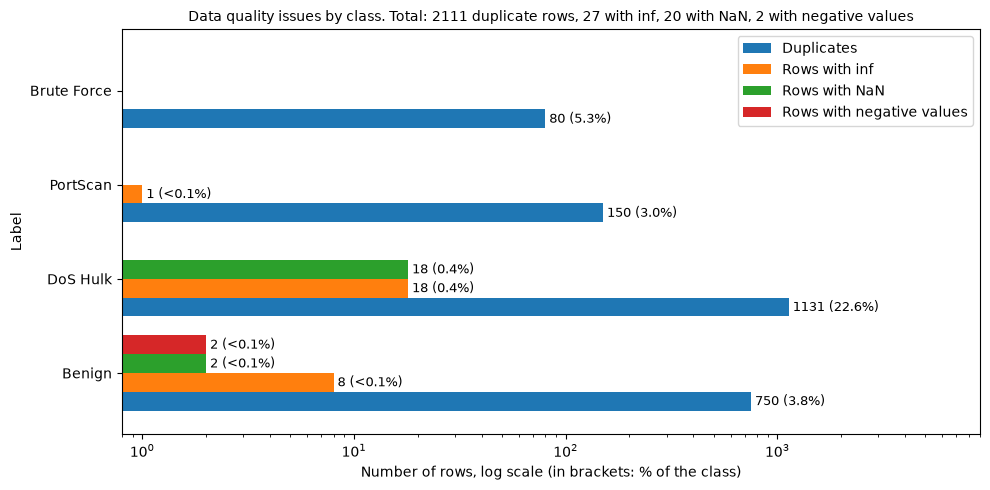
\includegraphics[width=0.68\textwidth]{figures/data_issues.png}
\caption{Data-quality issues per class (logarithmic horizontal axis). Duplicate rows dominate and
are concentrated in DoS Hulk; infinite and negative values are a handful of rows, invisible at
this scale but never zero.}
\label{fig:issues}
\end{figure}

\textbf{Split.} We split 70/15/15 with stratification and seed 42: 20,568 training, 4,408
validation and 4,408 test flows, with 214 Brute Force flows in both validation and test.

\qa{Given what you found about class balance, should the split be stratified? Why? Where did you
fit any scaler/normalizer, on which partition, and what goes wrong if you fit it on all the data?}
Yes. Brute Force is 4.8\% of the data, so a random split can move a sizeable number of its 1,427
flows from one partition to another. With the same seed, the stratified split keeps the Brute
Force share within 0.01 points across the three sets (4.86\%, 4.85\%, 4.85\%), while the random
split moves it between 4.45\% and 4.97\% (Figure~\ref{fig:split}), i.e.\ about 40 flows more in
validation and 22 fewer in test; the direction depends on the seed, the variance is the problem.
The scaler is fitted on the training partition only and then applied to validation and test.
\texttt{log1p} learns no parameter, but \texttt{StandardScaler} learns a mean and a standard
deviation: if it were fitted on all the data, those statistics would also depend on the test set,
information from the test set would leak into training, and the test score would stop being an
honest estimate on unseen traffic.

\begin{figure}[htbp]
\centering
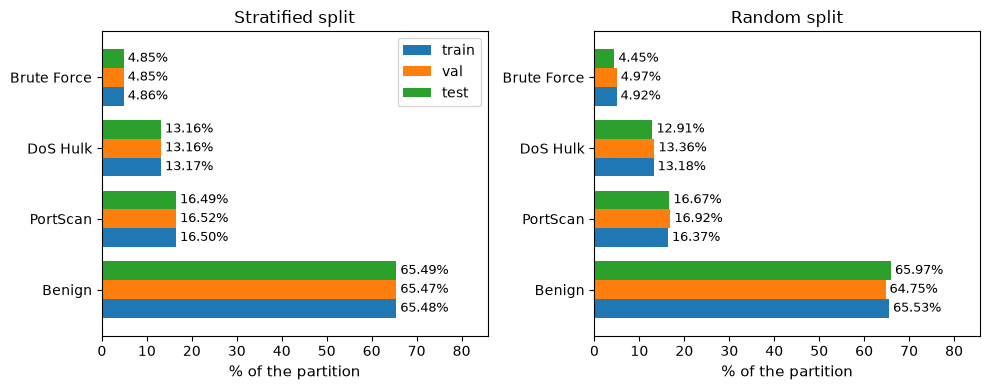
\includegraphics[width=0.72\textwidth]{figures/split.png}
\caption{Share of each class in the three partitions with a stratified split (left) and with a
random split using the same seed (right). Stratification keeps the proportions constant; the
random split moves Brute Force between partitions.}
\label{fig:split}
\end{figure}

\qa{Which scaling did you pick and why? How did the outliers inform the choice?}
\texttt{log1p} followed by \texttt{StandardScaler}, fitted on the training set. The raw features
span very different ranges: the flag counters are 0/1, the number of forward packets has median 2
and maximum 3,141, \texttt{Flow Duration} reaches $1.2\cdot10^{8}$ and \texttt{Flow Bytes/s}
$2.1\cdot10^{9}$. These extremes are plausible flows (long sessions, attack traffic), so we kept
them instead of clipping them, and compared three scalers (Figure~\ref{fig:scaling}).
\texttt{StandardScaler} alone divides by a standard deviation inflated by the tails: the central
50\% of the features is squeezed into a median IQR of 0.16 and the largest value still reaches 85,
so most of the data collapses around zero. \texttt{RobustScaler} keeps the bulk well spread (median
IQR 1.00) but does not change the shape of the distribution, so the tails still reach 13,957 scaled
units and a few flows dominate the gradient. \texttt{log1p} attacks the cause: the features are
counts, durations and rates with long right tails, and the logarithm makes them roughly symmetric
before standardisation, leaving a usable dynamic range (median IQR 1.55, largest value 9). It has no
parameters and every value is non-negative after cleaning, so applying it to all partitions causes
no leakage.

\begin{figure}[htbp]
\centering
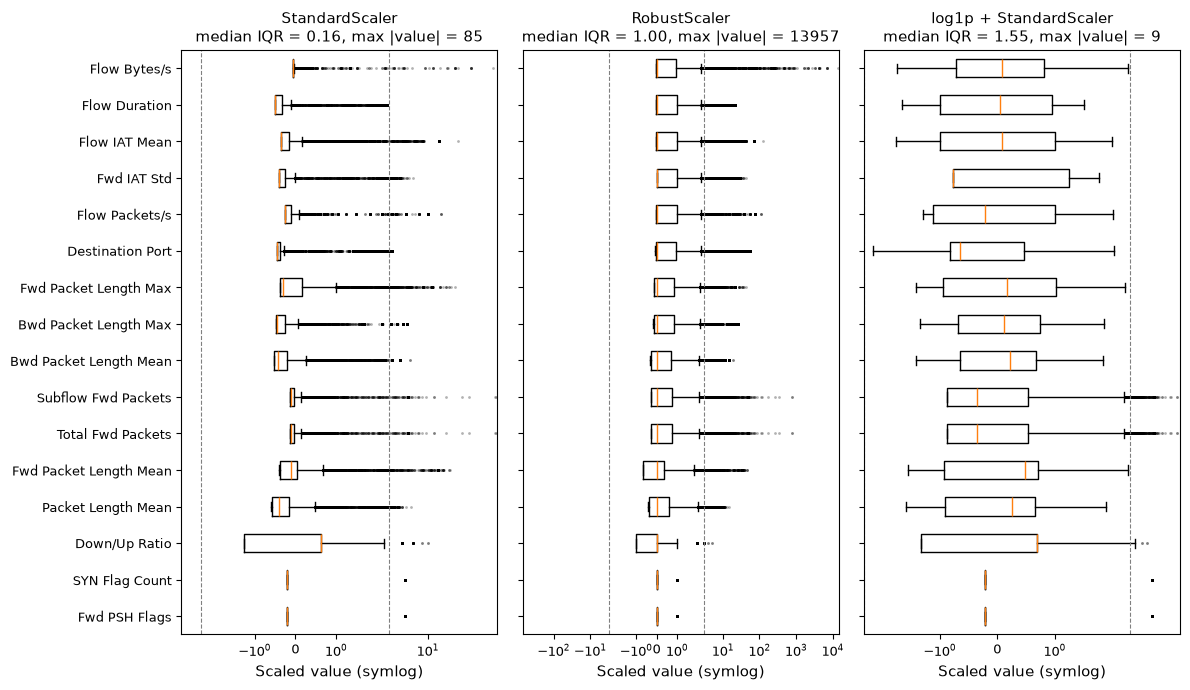
\includegraphics[width=0.88\textwidth]{figures/scaling.png}
\caption{Distribution of each feature in the training set after the three scaling options
(boxplots, symmetric-log axis, dashed lines at $\pm3$). Panel titles report the median IQR and the
largest absolute value. Only \texttt{log1p}+\texttt{StandardScaler} spreads the bulk of the data
without leaving extreme values.}
\label{fig:scaling}
\end{figure}

% ===========================================================================
\section{Task 2 -- A first network}

\subsection{Task 2A -- Baseline}
\textbf{Setup.} One hidden layer of 64 units, ReLU, cross-entropy loss, AdamW with learning rate
$5\cdot10^{-4}$ and weight decay 0.01, batch size 64, at most 100 epochs, early stopping on the
validation loss (patience 10, $\min\Delta=10^{-5}$, best weights restored), seed 42. These are the
values suggested by the lab; we keep them unchanged so that \run{R1} is a simple, reproducible
reference.

\textbf{Prediction (before running).} Brute Force is the hardest class, with the lowest
\emph{recall}: it is 4.8\% of the data and the loss has no class weights, so the network should
favour the majority class.

\qa{How do you pick the ``best'' model across epochs? Do the curves converge?}
We keep the weights of the epoch with the lowest validation loss, checked after every epoch, with
patience 10 and the best weights restored at the end. We use the loss rather than the macro-F1
because the loss is what the network minimises and it changes smoothly, while the macro-F1 jumps
from one epoch to the next when a single rare flow changes side (Figure~\ref{fig:r1}, right). The
curves do converge: both losses fall quickly in the first 20 epochs and then decrease very slowly,
ending within 0.001 of each other (0.027 training, 0.028 validation), so there is no overfitting.
Early stopping never fired: the best epoch is 96 of 100, so the curve was still improving
marginally when the budget ended.

\begin{figure}[htbp]
\centering
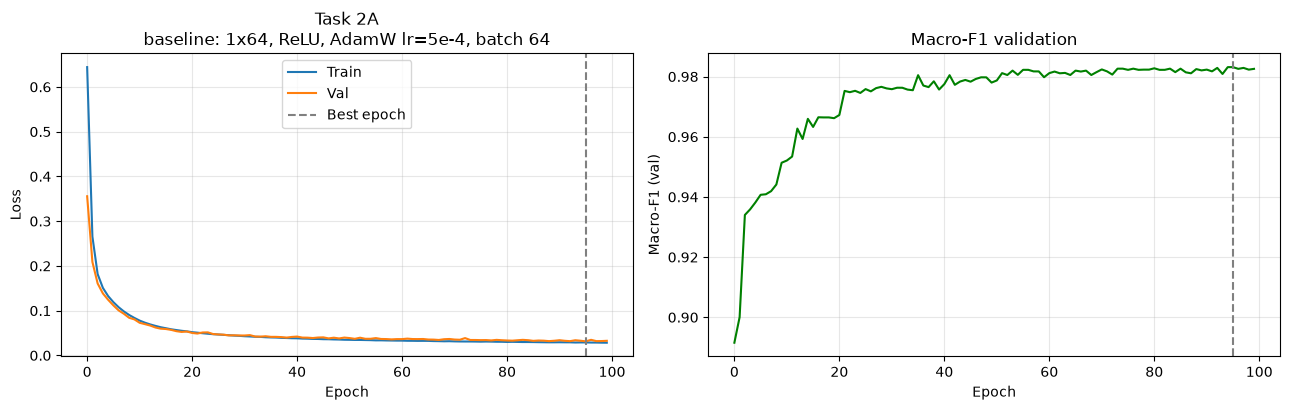
\includegraphics[width=0.90\textwidth]{figures/r1_curves.png}
\caption{\run{R1} (baseline). Left: training and validation loss. Right: validation macro-F1. The
dashed line marks the best epoch (96). The two losses stay together and are still slowly
decreasing at epoch 100.}
\label{fig:r1}
\end{figure}

\qa{Do your hardest-class predictions hold up? Explain the per-class results.}
Only partly, and the way it fails is informative. Brute Force is indeed the weakest class, with
F1 0.953 against at least 0.988 for the others (Table~\ref{tab:r1}), but its \emph{recall} is the
highest of all (0.995: 213 of 214 flows found) and its \emph{precision} the lowest (0.914). The
errors therefore go the other way: 20 Benign flows are classified as Brute Force and 9 as DoS
Hulk, while only one Brute Force flow is missed. So the rare class is not ignored: the model finds
nearly all of it and pays with false positives. Brute Force is not hard because it is rare, but
because some Benign flows look like it, so the network must be using a feature that the two classes
share. Task~3 tests the obvious candidate, the destination port.

\begin{table}[htbp]
\centering\small
\caption{\run{R1} validation classification report (accuracy 0.992, macro-F1 0.983). Brute Force
has the highest recall and the lowest precision.}
\label{tab:r1}
\begin{tabular}{@{}lrrrr@{}}
\toprule
Class & Precision & Recall & F1 & Support\\
\midrule
Benign       & 0.999 & 0.990 & 0.994 & 2,886\\
Brute Force  & 0.914 & 0.995 & 0.953 &   214\\
DoS Hulk     & 0.980 & 0.997 & 0.988 &   580\\
PortScan     & 0.999 & 0.996 & 0.997 &   728\\
\midrule
Macro avg    & 0.973 & 0.994 & 0.983 & 4,408\\
\bottomrule
\end{tabular}
\end{table}

\subsection{Task 2B -- Why the fundamentals matter}
Each run starts from \run{R1} and changes one thing (Table~\ref{tab:2b}, Figure~\ref{fig:2b}).

\qa{Rank S1--S3 by how badly they hurt, and say which fundamental -- scaling or the learning rate
-- you would get right first on a new problem.}
By validation macro-F1 the ranking is S3 (0.893) $<$ S2 (0.910) $<$ S1 (0.921), against 0.983 for
\run{R1}; Brute Force F1 falls in the same order (0.814, 0.770, 0.846), so the ranking is not an
artefact of one class. We would fix \emph{scaling} first. It is a property of the data that no
learning rate can compensate: with features spanning $10^{0}$ to $10^{9}$ the same step is
enormous for one feature and negligible for another, and the network needs a much larger budget to
recover. The learning rate is the second knob, because it is cheap to sweep and, as S3 shows, the
cost of a wrong value is an unconverged model.

\qa{Suppose you were handed just one of these loss curves, with no note of what had been changed.
What in the shape of the curve would point you to the cause?}
Three signatures, all visible in Figure~\ref{fig:2b}. \emph{Scale}: an untrained network over four
classes has a loss of about $\ln 4\approx1.4$, so a first loss of $\sim$80,000 (panel a) says the
inputs are unscaled, and the curve then keeps jumping because the large-range features dominate the
gradient. \emph{Oscillation}: a loss of normal size that goes up and down instead of down, with
the validation loss spiking to 22 and a best epoch of 5 (panel b), says the learning rate is too
high: every step overshoots the minimum, and AdamW only caps the size of the step, which is why
the loss oscillates instead of exploding. \emph{A smooth curve that never converges}: a loss that
decays regularly but is still at 0.3 when the budget ends (panel c), with training and validation
almost on top of each other, says the learning rate is too low: the direction is right and the
progress per step is 100 times too small. Panel (c) already reaches macro-F1 0.9 at epoch 100: the
classification metric hides how far the model is from the minimum, another reason to read the loss
curve.

\begin{table}[htbp]
\centering\small
\caption{Task 2B, one change per run from \run{R1} (validation). The last column gives the best epoch
over the epochs actually run, i.e.\ where early stopping stopped the training.}
\label{tab:2b}
\begin{tabular}{@{}llrrrr@{}}
\toprule
Run & Change & Macro-F1 & BF F1 & BF recall & Best epoch\\
\midrule
\run{R1} & baseline                    & 0.983 & 0.953 & 0.995 &  96/100\\
\run{R2} & S1: no scaling              & 0.921 & 0.846 & 0.836 &  46/56\\
\run{R3} & S2: lr $5\cdot10^{-4}\to0.5$  & 0.910 & 0.770 & 0.836 &   5/15\\
\run{R4} & S3: lr $5\cdot10^{-4}\to5\cdot10^{-6}$ & 0.893 & 0.814 & 0.836 & 100/100\\
\bottomrule
\end{tabular}
\end{table}

\begin{figure}[htbp]
\centering
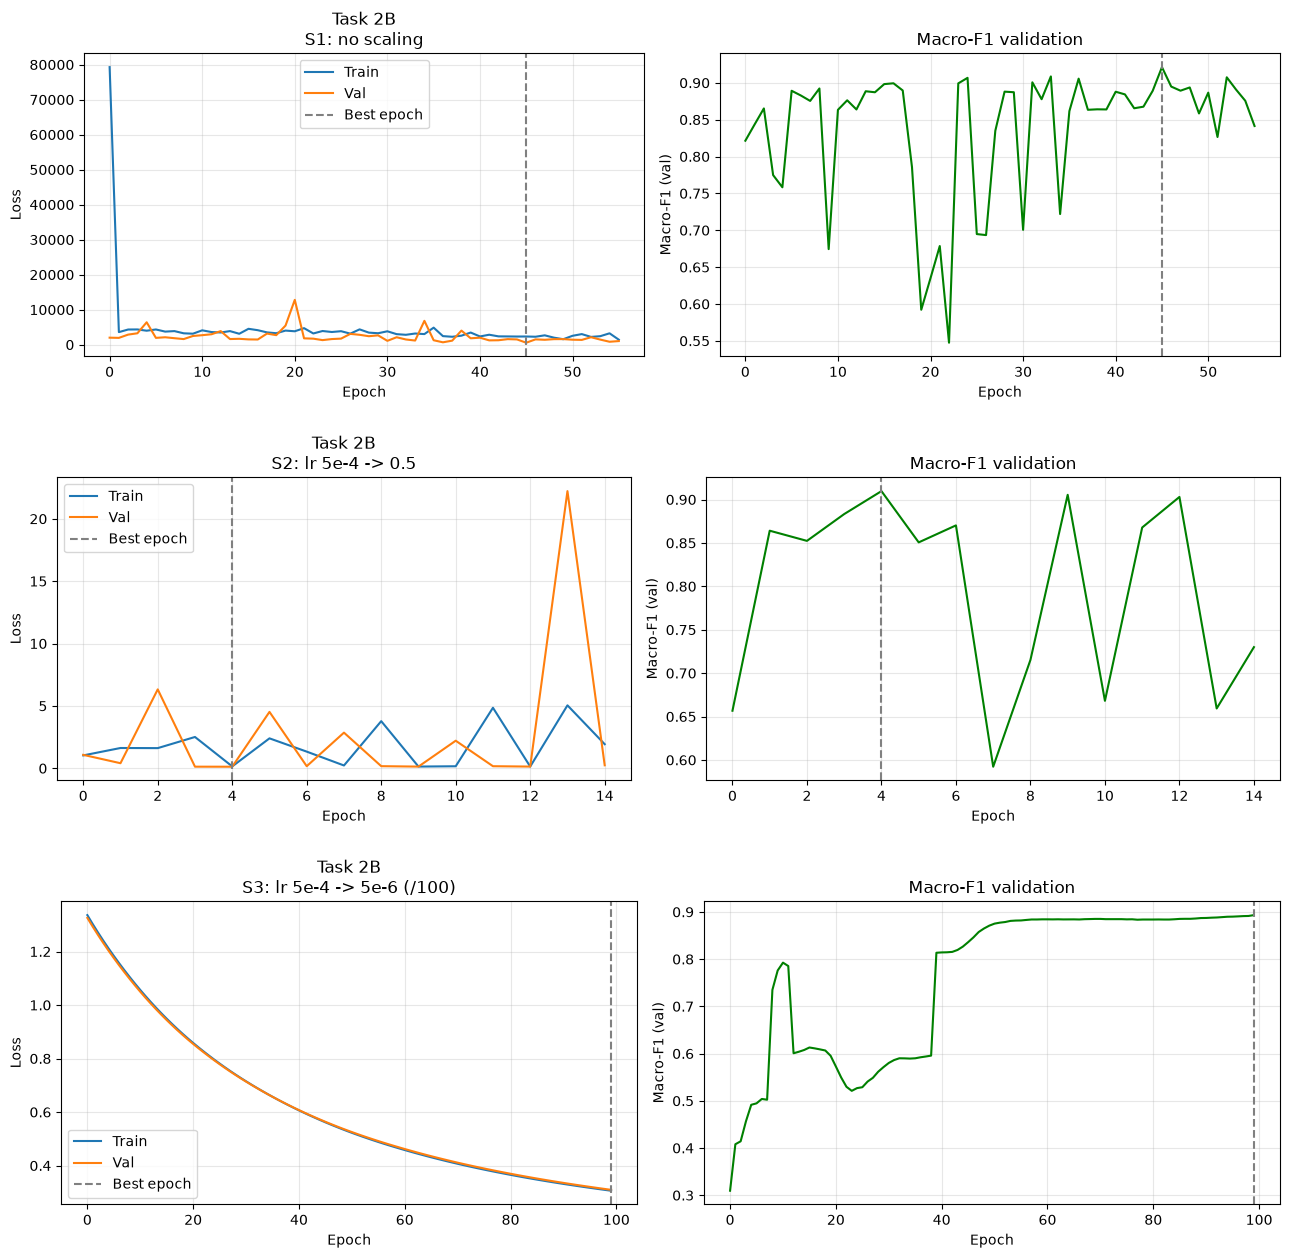
\includegraphics[width=0.70\textwidth]{figures/r2_r3_r4_curves.png}
\caption{Loss and validation macro-F1 of the three failure modes, same layout as
Figure~\ref{fig:r1}: (a) S1, no scaling, initial loss $\sim$80,000; (b) S2, learning rate 0.5,
oscillating loss, best epoch 5; (c) S3, learning rate $5\cdot10^{-6}$, slow monotone descent still
far from the minimum at epoch 100.}
\label{fig:2b}
\end{figure}

\subsection{Task 2C -- Final baseline}
\run{R5} repeats \run{R1} with 300 epochs, since \run{R1} was still improving at epoch 96 of 100. It
reaches the same 0.983 macro-F1 (best epoch 156 of 166): the extra budget bought stability, not
accuracy, and we keep it as the baseline to beat. \run{R6} then changes the activation to linear.

\qa{Compare validation vs test. Does it generalize (is the gap small)?}
Yes (Table~\ref{tab:2c}). Validation: accuracy 0.992, macro-F1 0.983, loss 0.0273. Test: accuracy 0.992, macro-F1 0.983,
loss 0.0282. The gaps are +0.0009 in loss and $-0.0003$ in macro-F1, Brute Force recall is 0.995 on
validation and 1.000 on test, and no class moves by more than 0.001. A model trained once on 20,568
flows and evaluated on 4,408 unseen ones reproduces its validation score, so there is no
overfitting to the validation set and the split is sound.

\qa{Does switching the activation (ReLU $\to$ linear, \run{R6}) change per-class behaviour? Would it
be fair to compare these two on the test set, or is the test set off-limits for choosing between
them? Why?}
Yes, and selectively: macro-F1 drops from 0.983 to 0.922, driven by Brute Force (F1 0.953 $\to$
0.797, recall 0.995 $\to$ 0.836) and DoS Hulk (0.988 $\to$ 0.922), while PortScan barely moves
(0.997 $\to$ 0.992) and accuracy stays at 0.962. The two classes that lose the most are exactly the
two that live on port 80, which is what a linear model cannot separate from the Benign traffic that
also uses port 80 (10.5\% of the Benign flows). Comparing them on the test set would be unfair: the
choice between ReLU and linear is a model-selection decision, so it belongs to validation. Using
test to pick the winner would make it part of the selection and its score would no longer estimate
performance on new traffic.

\begin{table}[htbp]
\centering\small
\caption{Task 2C: the 300-epoch baseline \run{R5} on validation and test, and the linear-activation
variant \run{R6} on validation.}
\label{tab:2c}
\begin{tabular}{@{}lrrrr@{}}
\toprule
Model / split & Accuracy & Macro-F1 & BF F1 & DoS F1 \\
\midrule
\run{R5} validation (300 epochs) & 0.992 & 0.983 & 0.953 & 0.989\\
\run{R5} test                     & 0.992 & 0.983 & 0.953 & 0.987\\
\run{R6} validation (linear)      & 0.962 & 0.922 & 0.797 & 0.922\\
\bottomrule
\end{tabular}
\end{table}

% ===========================================================================
\section{Task 3 -- When a feature biases the model}

\qa{Is ``Brute Force always on port 80'' a property of brute-force attacks in general, or an artefact
of this dataset? If your model sees this, what is it likely to learn?}
It is an artefact of how this dataset was collected and labelled, not a property of brute-force
traffic: a brute-force attempt against SSH, FTP or a web login form runs on a different port, and
port 80 is simply where this capture placed it. The measurement confirms how clean the shortcut is:
100\% of the Brute Force flows and 100\% of the DoS Hulk flows are on port 80, against 10.5\% of the
Benign flows and 0.1\% of the PortScan flows. A model that sees the port can therefore separate
Brute Force from 89.5\% of Benign with a single threshold on one input, and it will learn exactly
that: the port, not the traffic shape. The evidence was already in Task~2A, where the only Brute
Force errors were false positives on the 10.5\% of Benign flows that share the port, and where the
linear model lost most of its accuracy on the same two classes.

\qa{(Counterfactual, after running) Did your prediction hold? What does this reveal about what the
model was really using to detect Brute Force?}
Prediction (written before running): Brute Force recall would collapse, because the model never
learned to recognise the traffic, only the port. It held, completely. We moved the 214 Brute Force
test flows from port 80 to port 8080 and re-ran inference with \run{R5}, without retraining: recall
1.000 $\to$ 0.000 (F1 0.000), accuracy 0.992 $\to$ 0.943, macro-F1 0.983 $\to$ 0.736, and the
unweighted loss jumps from 0.028 to 0.903. Benign, DoS Hulk and PortScan are essentially unchanged
(recall 0.989, 0.997, 0.997), and all 214 Brute Force flows are now predicted Benign
(Figure~\ref{fig:cf}). A single column changed, no retraining, and the class disappears: the model
was reading the destination port.

\begin{figure}[htbp]
\centering
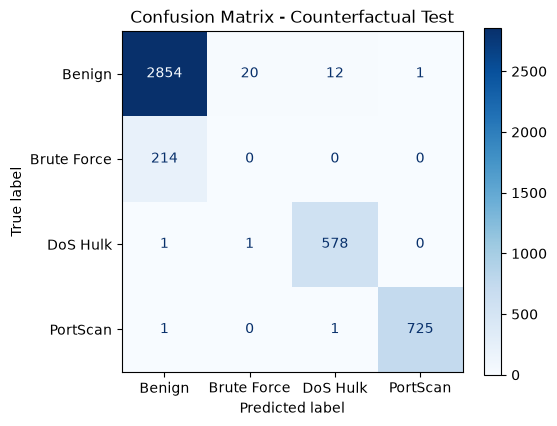
\includegraphics[width=0.42\textwidth]{figures/cm_counterfactual.png}
\caption{Counterfactual test with \run{R5}: only the destination port of the Brute Force flows
changed (80 $\to$ 8080). The Brute Force row has no correct prediction left.}
\label{fig:cf}
\end{figure}

\textbf{The port-free dataset.} We remove \texttt{Destination Port} and redo cleaning, split and
scaling. Table~\ref{tab:t3} compares three datasets: \run{D} (with the port, de-duplicated),
\run{D1} (port removed, no deduplication) and \run{D2} (port removed, de-duplicated), which is the
one used from Task~4 on. \run{D2} keeps 22,468 flows: 15,727 training, 3,370 validation, 3,371
test.

\qa{Count your classes after cleaning now, and compare to before. One class shrinks dramatically
when you remove the port and de-duplicate. Which one, and by how much?}
PortScan, by 94.1\%: 4,849 flows in \run{D}, 285 in \run{D2}. Benign loses 12.2\%, while DoS Hulk
and Brute Force end at exactly their \run{D} counts: the extra rows that appear in \run{D1} are
duplicates that only exist once the port is removed, and deduplication removes them again.

\qa{Why does that class collapse while the others barely move? What does that tell you about what
the model ``knew'' about that class before you removed the port?}
Because a port scan is, by definition, the same connection attempt repeated on many different
ports. With the port in the features every probe is a different flow; without it, 4,714 of the 4,999
PortScan flows become exact duplicates of one another and disappear. Brute Force and DoS Hulk
barely move because their flows differ in size, duration and rate, not only in the port. What the
model \emph{knew} about PortScan was therefore mostly the port value itself: the class had very
little intrinsic variety to learn. This is the same failure as in the counterfactual, in the
opposite direction: the model was rewarded for reading an input that identifies the class rather
than describing it.

\qa{After dropping the port, which class is now the rarest? How balanced is the data now?}
PortScan, with 285 flows (1.3\% of \run{D2}); Brute Force is now the second rarest with 1,427
(6.4\%), Benign is 75.2\% and DoS Hulk 17.2\%. The problem is \emph{more} imbalanced than before in
terms of the rarest class, while the biggest class has grown from 65.5\% to 75.2\% of the data. In
absolute terms, validation and test contain 43 PortScan flows each: one flow moves their recall by
2.3 points, and this is the reason why we treat differences below $\sim$0.05 macro-F1 as noise.

\qa{Knowing that de-duplication decimates one class once the port is gone, do you still de-duplicate?
Argue your choice.}
Yes. The alternative is to keep 4,714 copies of a handful of PortScan flows, which is worse for two
reasons: the model would be trained and tested on the same flows (the leakage argument of Task~1),
and the class would look 17 times larger than the number of distinct behaviours it contains, so any
score on it would be an artefact of counting. Deduplicating makes the task harder but honest: 285
distinct flows are still 285 different behaviours, and \run{R7} shows that the class remains
detectable (validation recall 0.907). The cost of this choice is measured, not hidden: it is the
0.024 macro-F1 that the port-free, de-duplicated baseline loses with respect to \run{R5}.

\begin{table}[htbp]
\centering\small
\caption{Class counts in the three versions of the dataset. \run{D2} is used from Task~4 on; the
last column is the share of each class lost between \run{D} and \run{D2}.}
\label{tab:t3}
\begin{tabular}{@{}lrrrr@{}}
\toprule
Class & \run{D} with port & \run{D1} no port & \run{D2} no port + dedup & Lost vs \run{D}\\
\midrule
Benign       & 19,240 & 19,990 & 16,888 & 12.2\%\\
Brute Force  &  1,427 &  1,507 &  1,427 &  0.0\%\\
DoS Hulk     &  3,868 &  4,982 &  3,868 &  0.0\%\\
PortScan     &  4,849 &  4,999 &    285 & 94.1\%\\
\midrule
Total        & 29,384 & 31,478 & 22,468 & 23.5\%\\
\bottomrule
\end{tabular}
\end{table}

% ===========================================================================
\section{Task 4 -- The rare class}

\textbf{Prediction (before running).} PortScan will suffer most, because after removing the port and
the duplicates only 285 distinct flows are left. \run{R7} retrains the Task~2C baseline on \run{D2}
with the same hyper-parameters (1$\times$64, ReLU, AdamW, 300 epochs). Validation macro-F1 falls
from 0.983 to 0.959 and PortScan recall to 0.907: the prediction was right in direction and wrong
in magnitude, the class is still detected.

\qa{Can you still detect the rarest class at all?}
Yes. On validation PortScan reaches precision 0.975, recall 0.907 and F1 0.940 on 43 flows, with
overall accuracy 0.982 and macro-F1 0.959 (Table~\ref{tab:t4}). The class is rare but not lost: its
distinct flows remain different from the other traffic once the port is gone. The loss with respect
to the port-aware baseline (0.983) is 0.024 macro-F1, and most of it is PortScan and Brute Force.

\qa{From which partition do you compute the class weights, and why would using any other partition
be wrong?}
From the training split of \run{D2} only, with $\mathrm{weight}_c = N/(K\,n_c)$ over the 15,727
training flows: Benign 0.33, Brute Force 3.94, DoS Hulk 1.45, PortScan 19.76. Weights computed on
validation or test would encode the evaluation distribution into the loss: the model would be
optimised for the set used to judge it, the numbers would be optimistic, and the weights could not
be reproduced on new traffic whose composition we do not know.

\qa{(After running \run{R8}) Did accuracy and macro-F1 move in the same direction? For an intrusion
detector that must catch rare attacks, which metric should you optimize, and why?}
Yes, both fell: accuracy 0.982 $\to$ 0.960 and macro-F1 0.959 $\to$ 0.884.
What the weights bought is recall: PortScan 0.907 $\to$ 0.977, Brute Force 0.939 $\to$ 0.986, DoS
Hulk 0.967 $\to$ 0.979. What they cost is precision on the rarest class: PortScan 0.975 $\to$ 0.553,
i.e.\ 34 false alarms on 2,533 Benign flows instead of 1. This is the expected trade, and it does not
help macro-F1, which averages precision and recall. For an intrusion detector the metric to optimise
is rare-class \emph{recall} (or macro-F1 as a compromise): accuracy is dominated by Benign (75\% of
the flows) and can be high while the detector misses the attacks it exists for. A missed attack and
a false alarm do not have the same cost, so the right output is not a single number but an operating
point chosen on the precision/recall curve; with 43 PortScan flows in validation, we can only state
the trade, not tune it finely.

\begin{table}[htbp]
\centering\small
\caption{Task 4 on validation (3370 flows, 43 PortScan). \run{R7} keeps the unweighted loss,
\run{R8} adds the balanced class weights; everything else is identical.}
\label{tab:t4}
\begin{tabular}{@{}lrrrrr@{}}
\toprule
Run & Accuracy & Macro-F1 & PortScan P / R / F1 & Brute Force F1 & Benign recall\\
\midrule
\run{R7} unweighted & 0.982 & 0.959 & 0.975 / 0.907 / 0.940 & 0.935 & 0.990\\
\run{R8} weighted   & 0.960 & 0.884 & 0.553 / 0.977 / 0.706 & 0.904 & 0.953\\
\bottomrule
\end{tabular}
\end{table}

% ===========================================================================
\section{Task 5 -- Varying the hyper-parameters}

\textbf{Budget.} 10 runs: 3 for depth (5A), 3 for batch size (5B), 4 for optimizer and learning
rate (5C). Every run is one change from a stated parent, and every hypothesis was written before
running (Appendix~A).

\subsection{5A -- Depth}
We chose three configurations instead of a grid: (64,32) adds one layer to the baseline,
(64,32,16) adds a narrower third layer, and (128,64,32) widens that three-layer network, so depth
and width are measured separately. All three keep the balanced loss and 300 epochs of \run{R8}.

\qa{Does depth help on this problem? If a single-hidden-layer baseline stays competitive, what does
that suggest about the complexity of this task?}
The second layer helps a little (+0.017, 0.884 $\to$ 0.901), the third one hurts ($-$0.004,
0.897), and the only configuration that clearly improves is the wider one (0.925, +0.028 over the
three-layer (64,32,16) and +0.041 over the single layer, Table~\ref{tab:t5}). Width, not depth, is
the lever, and even the best Task~5 model stays below the \emph{unweighted} single-layer baseline of
Task~4 (0.959): the effect of depth is smaller than the effect of the loss function. This suggests a
low-dimensional, largely separable task in which a single hidden layer already has enough capacity,
and where the remaining errors come from the overlap between classes (Benign on port 80) rather
than from missing interactions.

\subsection{5B -- Batch size}
We bracket the two extremes: 16, 128 and 1024, all on the 1$\times$64 weighted baseline.

\qa{Report validation results and training time, and explain both.}
At batch 16 the model generalises best (0.899) and is by far the slowest: 133.5 s for 60 epochs, 2.2 s
per epoch, because each epoch contains 983 weight updates instead of 123 or 16. At batch 128 it
reaches 0.868 in 45.2 s, and at 1024 0.866 in 48.7 s with 300 epochs (Table~\ref{tab:t5}). The
largest batch is not the fastest overall: its epochs are cheap (0.16 s) but it needs almost three
times as many of them (300 against 109), so the wall-clock time is the same as batch 128. The gain
of small batches is real but small, and it comes with more updates: with 15,727 training flows per
epoch, batch 1024 sees
only $\sim$4,800 updates in 300 epochs against $\sim$59,000 for batch 16, so part of the gap is an
optimization budget, not the batch size itself. The two-worst configurations differ by 0.002, which
is inside the noise of 43 PortScan flows: only the ordering of the times is solid.

\subsection{5C -- Optimizer vs.\ learning rate}
Four runs on the same 1$\times$64 weighted model: SGD at 0.01, SGD at 0.1, SGD with momentum 0.9 at
0.01, and AdamW at $5\cdot10^{-3}$. All of them use the same weight decay 0.01.

\qa{What did you find -- does the optimizer or the learning rate dominate on this data?}
Neither, cleanly, and the runs cannot fully separate them. Inside SGD the learning rate is the main
lever: multiplying it by 10 takes macro-F1 from 0.787 to 0.817 (+0.030) and the run from 130 to 27
epochs; momentum at the badly chosen learning rate changes nothing measurable (0.781, $-$0.006),
because it cannot compensate for a step that is too small. But at the same weight decay AdamW reaches
0.897, +0.080 over the best SGD, so here the optimizer/weight-decay combination moves the result much
more than any learning-rate step \emph{inside} the family. Two honest caveats. \run{R18} changes the
optimizer \emph{and} the learning rate (10$\times$ higher than \run{R8}), so it cannot attribute the
gain to either. And weight decay is not the same operation in the two optimizers: AdamW applies it
directly to the weights, while in SGD it is an L2 term added to the gradient, which at learning rate
0.01 is a strong pull towards zero. The SGD runs at 0.787--0.817 are therefore not a fair picture of
SGD, they are a picture of SGD with a regularisation it cannot afford.

\subsection{5D -- Verdict}
\qa{Did the added complexity beat the simple baseline? Was it worth the runs it cost?}
No. On test, the simple port-free baseline \run{R7} reaches macro-F1 0.957 and accuracy 0.980, while
the best Task~5 model \run{R11} reaches 0.928 and 0.966 (Table~\ref{tab:5d}). Complexity does not beat
the baseline: it only recovers part of what the class weights had cost (\run{R8} is 0.871). The
per-class detail says the same: \run{R11} finds PortScan more often (recall 0.977 vs 0.884) but with
many more false alarms (precision 0.808 vs 0.974), and it is worse on Brute Force (F1 0.895 vs 0.949).
Ten runs of Task~5 produced no model better than the 1$\times$64 network of Task~4: the architecture
was not the bottleneck, and the runs were not worth it beyond what we learned about depth, batch size
and optimizers.

\begin{table}[htbp]
\centering\small
\caption{Task 5 on validation (3370 flows). All runs use the balanced loss and 300 epochs; 5B and
5C start from the 1$\times$64 weighted baseline \run{R8}. Times are wall-clock seconds for the whole
run on the same GPU.}
\label{tab:t5}
\begin{tabular}{@{}llrrrr@{}}
\toprule
Run & Change & Macro-F1 & Accuracy & Best epoch & Time (s)\\
\midrule
\run{R9}  & 5A: hidden (64,32)          & 0.901 & 0.963 &  32/42  & 28.3\\
\run{R10} & 5A: hidden (64,32,16)       & 0.897 & 0.962 &  33/43  & 31.9\\
\run{R11} & 5A: hidden (128,64,32)      & 0.925 & 0.969 &  22/32  & 25.5\\
\midrule
\run{R12} & 5B: batch 16                & 0.899 & 0.965 &  50/60  & 133.5\\
\run{R14} & 5B: batch 128               & 0.868 & 0.957 &  99/109 &  45.2\\
\run{R13} & 5B: batch 1024              & 0.866 & 0.954 & 293/300 &  48.7\\
\midrule
\run{R15} & 5C: SGD lr 0.01             & 0.787 & 0.906 & 120/130 &  88.8\\
\run{R16} & 5C: SGD lr 0.1              & 0.817 & 0.920 &  17/27  &  13.6\\
\run{R17} & 5C: SGD + momentum, lr 0.01 & 0.781 & 0.905 &  60/70  &  36.3\\
\run{R18} & 5C: AdamW lr $5\cdot10^{-3}$  & 0.897 & 0.964 &  21/31  &  17.9\\
\bottomrule
\end{tabular}
\end{table}

\begin{table}[htbp]
\centering\small
\caption{Task 5D: the test-set comparison (3371 flows) between the simple port-free baseline and the
best Task~5 model. The test set is used once, for this verdict.}
\label{tab:5d}
\begin{tabular}{@{}lrrrr@{}}
\toprule
Model & Macro-F1 & Accuracy & PortScan P / R & Brute Force F1\\
\midrule
\run{R7} 1$\times$64, unweighted (baseline) & \textbf{0.957} & \textbf{0.980} & 0.974 / 0.884 & 0.949\\
\run{R11} (128,64,32), weighted             & 0.928 & 0.966 & 0.808 / 0.977 & 0.895\\
\run{R8} 1$\times$64, weighted               & 0.871 & 0.952 & 0.532 / 0.977 & 0.889\\
\bottomrule
\end{tabular}
\end{table}

% ===========================================================================
\section{Task 6 -- Optimizations}

\textbf{Setup (\run{R19}).} Five hidden layers of 256-128-64-32-16 units, ReLU, cross-entropy,
AdamW $5\cdot10^{-4}$, batch 128, 200 epochs, no regularization and no early stopping.
\textbf{Prediction (before running).} The capacity is far larger than the task: the training loss
will keep falling while the validation loss flattens after a few dozen epochs.

\qa{Is it overfitting? Show exactly where you see it in the curves.}
Yes, mildly, and the curves show where. Up to epoch $\sim$45 the training and validation losses fall
together; the minimum of the validation loss is at epoch 44. After that the training loss keeps
falling to $\sim$0.03 while the validation loss climbs steadily to $\sim$0.19 at epoch 200
(Figure~\ref{fig:6a}): the last 150 epochs only make the model fit the training flows. The
classification metric stays flat (the final model still scores 0.951), but the per-class table shows
where the memorisation is: PortScan recall is 1.000 on training and 0.954 on validation, so the
network memorises a few rare flows rather than the whole dataset. One caveat we checked: the loss
printed by \texttt{eval\_split} is unweighted, while the curves use the weighted criterion of
\texttt{fit}. On the final model the unweighted loss is 0.058 on training and 0.072 on validation, a
gap of only 0.014, while the weighted validation loss doubles after epoch 44: the rare classes it
weights are exactly the ones being memorised.

\begin{figure}[htbp]
\centering
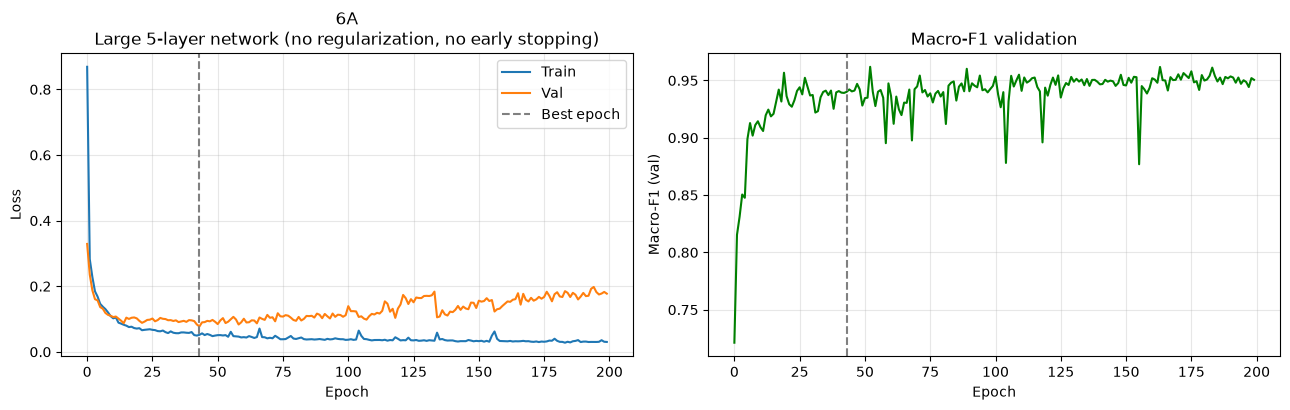
\includegraphics[width=0.90\textwidth]{figures/r19_curves.png}
\caption{\run{R19}: weighted training and validation loss (left) and validation macro-F1 (right).
The dashed line marks the minimum of the validation loss (epoch 44). The validation loss then rises
from 0.072 to $\sim$0.19 while the training loss keeps falling: the overfitting starts there.}
\label{fig:6a}
\end{figure}

\textbf{Optimising it.} One change per run, simplest first (Table~\ref{tab:t6}): early stopping
(\run{R20}), then weight decay on top of it (\run{R21}), then dropout (\run{R22}), then batch
normalization (\run{R23}); finally, the other half of the first countermeasure, a much smaller
network (\run{R24}, 1$\times$64, same protocol).

\qa{Which change helped the most for the least effort?}
Early stopping, by a wide margin: it cuts the run from 200 to 25 epochs (4.9 s instead of 129 s) and
keeps validation macro-F1 at 0.919, 0.032 below the unregularized run. Among the regularizers, dropout
0.24 gives the best score (0.923, +0.004 over early stopping) for 10.5 s; weight decay adds nothing
measurable (0.921, +0.002) and batch normalization costs a run and lowers the score (0.907, $-$0.012
with respect to early stopping), which is what we predicted for such a small network. All the
differences between the regularized variants are within the noise of 43 PortScan flows. The ranking
is therefore: early stopping first, dropout if one more run is available, no batch normalization.

\qa{In the end, did the big network -- even with regularization -- do better on the test set than your
simple port-free baseline from Task 4?}
No, if the baseline is the model Task~4 actually ends with in its unweighted form, \run{R7}: on test
it reaches 0.957 macro-F1 and 0.980 accuracy, while the regularized five-layer network \run{R22}
reaches 0.929 / 0.964 and the small 1$\times$64 network \run{R24} 0.924 / 0.966
(Table~\ref{tab:test6}). Yes, if the comparison is with the weighted baseline \run{R8} (0.871 /
0.952), which is the model Task~4 ends with after the reweighting: \run{R22} gains +0.058. The
per-class detail explains the difference: the five-layer network finds PortScan more often (recall
1.000 vs 0.884) but with more false alarms (precision 0.827 vs 0.974), and it is slightly worse on
Brute Force (F1 0.882 vs 0.949). Regularization and early stopping recovered about two thirds of the
0.086 that the weighted loss had cost, but the plain 1$\times$64 unweighted network remains the best
model of the lab.

\qa{Final reflection: looking across the whole logbook, which decisions gave you the most performance
per unit of effort?}
The data decisions, not the models. \texttt{log1p}+\texttt{StandardScaler} is worth 0.062 macro-F1
(\run{R2} 0.921 $\to$ \run{R1} 0.983) for a few lines of code, and no architecture change came
close: none of them improved the baseline by more than 0.041. Stratification does not change the
mean score, but it removes a several-point swing in the share of a class that has 43 flows in test.
Removing the port cost 0.024 macro-F1, but it removed a shortcut that was worth all of Brute Force
recall (1.000 $\to$ 0.000 when only the port changed) and it is the decision that makes the rest of
the lab meaningful. Class weights bought rare-class recall (PortScan 0.907 $\to$ 0.977) at the price of
macro-F1 (0.959 $\to$ 0.884), a trade to decide with the deployment cost, not a free gain. The most
efficient run of all was early stopping: 25 epochs instead of 200 for 0.032 of validation macro-F1.

\begin{table}[htbp]
\centering\small
\caption{Task 6 on validation (3370 flows). \run{R19} is the unregularized reference; each following
run changes one thing from the previous one. Times are wall-clock seconds.}
\label{tab:t6}
\begin{tabular}{@{}llrrrr@{}}
\toprule
Run & Change & Macro-F1 & Accuracy & Best epoch & Time (s)\\
\midrule
\run{R19} & 5 layers, no regularization, 200 epochs & 0.951 & 0.979 &  44/200 & 129.0\\
\run{R20} & + early stopping (patience 10)          & 0.919 & 0.965 &  15/25  &   4.9\\
\run{R21} & + weight decay 0.01                     & 0.921 & 0.967 &  15/25  &   4.6\\
\run{R22} & + dropout 0.24                          & 0.923 & 0.969 &  42/52  &  10.5\\
\run{R23} & + batch normalization                   & 0.907 & 0.964 &  32/42  &   9.6\\
\run{R24} & 1$\times$64, no regularization          & 0.923 & 0.970 & 117/200 &  72.6\\
\bottomrule
\end{tabular}
\end{table}

\begin{table}[htbp]
\centering\small
\caption{Task 6 verdict on the test set (3371 flows): the Task~4 baselines against the regularized
five-layer network and the small one-layer network.}
\label{tab:test6}
\begin{tabular}{@{}lrrrr@{}}
\toprule
Model & Macro-F1 & Accuracy & PortScan P / R & Brute Force F1\\
\midrule
\run{R7} 1$\times$64, unweighted (Task~4 baseline) & \textbf{0.957} & \textbf{0.980} & 0.974 / 0.884 & 0.949\\
\run{R8} 1$\times$64, weighted                      & 0.871 & 0.952 & 0.532 / 0.977 & 0.889\\
\run{R22} 5-layer + dropout + weight decay         & 0.929 & 0.964 & 0.827 / 1.000 & 0.882\\
\run{R24} 1$\times$64, no regularization            & 0.924 & 0.966 & 0.768 / 1.000 & 0.893\\
\bottomrule
\end{tabular}
\end{table}

% ===========================================================================
\clearpage
\appendix
\section{Experiment logbook}

One row per run that trains a model; preprocessing and data-analysis decisions are in
Section~\ref{sec:task1} and in the notebook. Each run changes one element with respect to the run
given in brackets. Validation is the split used to choose every model; the test set appears only in
5D and in the final Task~6 verdict. The run identifiers match the variables \texttt{r1}--\texttt{r24} of the notebook.
Budget: 24 runs in total, of which 10 in Task~5 and 6 in Task~6.

{\scriptsize
\setlength{\tabcolsep}{3pt}
\renewcommand{\arraystretch}{1.15}
\begin{longtable}{@{}>{\raggedright\arraybackslash}p{1.3cm}>{\raggedright\arraybackslash}p{0.75cm}>{\raggedright\arraybackslash}p{3.0cm}>{\raggedright\arraybackslash}p{3.3cm}>{\raggedright\arraybackslash}p{2.4cm}>{\raggedright\arraybackslash}p{3.8cm}@{}}
\toprule
Run & Task & What I changed (one thing) & Hypothesis before running & Key result (val) & What I concluded\\
\midrule
\endfirsthead
\toprule
Run & Task & What I changed (one thing) & Hypothesis before running & Key result (val) & What I concluded\\
\midrule
\endhead
\bottomrule
\endfoot
\textbf{R1} & 2A & First baseline: 1 hidden layer of 64 units, ReLU, AdamW 5e-4, batch 64, $\le$100 epochs, early stopping. & PortScan is the easiest class (its flows share a port pattern); Brute Force is the hardest because it is the rarest (4.9\%) and its flows are short. & macro-F1 0.983, acc 0.992, best epoch 96/100 & Confirmed only in part: Brute Force has the lowest F1 (0.953) but a recall of 0.995, so rarity does not cost recalls; the low F1 comes from precision. The model can exploit port 80.\\
\textbf{R2} ($\leftarrow$R1) & 2B & S1: train on raw, unscaled features; everything else as 2A. & Features span 1e0 to 1e9, so the gradient is badly conditioned: slower, noisier descent and a worse plateau. & macro-F1 0.921, acc 0.953, best epoch 46/56, BF-F1 0.846 & Confirmed: validation macro-F1 falls from 0.983 to 0.921. Still far from catastrophic, because AdamW adapts the step per parameter; scaling remains the first fundamental to fix.\\
\textbf{R3} ($\leftarrow$R1) & 2B & S2: learning rate 5e-4 $\rightarrow$ 0.5 (1000$\times$). & The steps will overshoot the minimum: the loss oscillates, never settles and early stopping fires after a few epochs. & macro-F1 0.910, acc 0.953, best epoch 5/15, BF-F1 0.770 & Confirmed: the best epoch is 5 and the run stops after $\sim$15 epochs, but the final macro-F1 (0.910) is higher than S3's. A too-large lr is destructive, yet AdamW absorbs it better than expected.\\
\textbf{R4} ($\leftarrow$R1) & 2B & S3: learning rate 5e-4 $\rightarrow$ 5e-6 (100$\times$ smaller). & The loss will fall almost linearly and still be falling when the 100-epoch budget ends. & macro-F1 0.893, acc 0.933, best epoch 100/100, BF-F1 0.814 & Confirmed: the best epoch is the last one (100) and the curve is still decreasing. This is the worst of the three failures (macro-F1 0.893) because the model is far from converged.\\
\textbf{R5} ($\leftarrow$R1) & 2C & 300 epochs instead of 100, everything else as 2A. & The 2A run was still improving at epoch 96 of 100, so a longer budget should give a small gain. & macro-F1 0.983, acc 0.992, best epoch 156/166 & No measurable gain: the best value is the same (0.983 macro-F1). The model had already converged; the extra epochs only make the baseline more stable. Kept as the baseline to beat.\\
\textbf{R6} ($\leftarrow$R5) & 2C & Activation ReLU $\rightarrow$ linear, on the 300-epoch baseline. & The port-80 attack classes are separated by a threshold; a linear model should lose more on them than on the other classes. & macro-F1 0.922, acc 0.962, best epoch 93/103 & Confirmed: macro-F1 falls to 0.922 and Brute Force F1 to 0.797. The non-linearity pays exactly on the classes that a single linear cut cannot separate.\\
\textbf{R7} ($\leftarrow$R5) & 4 & Retrain the baseline on the port-free, de-duplicated data (D2), same hyper-parameters. & PortScan will suffer most: after removing the port and the duplicates only 285 distinct flows are left (1.3\% of D2). & macro-F1 0.959, acc 0.982, best epoch 167/177, PortScan recall 0.907 & Partly confirmed: macro-F1 drops from 0.983 to 0.959 and PortScan recall to 0.907, but the class is still detected. The loss of the port costs more than the loss of the duplicates.\\
\textbf{R8} ($\leftarrow$R7) & 4 & Class-weighted cross-entropy (weights from the training split), same model. & Accuracy will fall, macro-F1 will rise; rare-class recall up, rare-class precision down. & macro-F1 0.884, acc 0.960, best epoch 81/91, PortScan recall 0.977 & Only the second half held: accuracy 0.982 $\rightarrow$ 0.960 and macro-F1 0.959 $\rightarrow$ 0.884 both fall, while PortScan recall rises to 0.977 and its precision drops to 0.553. Reweighting buys recall, not macro-F1 on this data.\\
\textbf{R9} ($\leftarrow$R8) & 5A & Two hidden layers (64, 32), weighted loss, 300 epochs. & One more layer can model interactions between rates and flag counts, so a small gain over the single layer. & macro-F1 0.901, acc 0.963, best epoch 32/42 & Confirmed: macro-F1 0.884 $\rightarrow$ 0.901 (+0.017). Small but positive.\\
\textbf{R10} ($\leftarrow$R9) & 5A & Three hidden layers (64, 32, 16). & A third, narrower layer adds capacity where the data is low-dimensional; expect no gain and a risk of underfitting. & macro-F1 0.897, acc 0.962, best epoch 33/43 & Confirmed: 0.897, slightly below the two-layer net. Depth alone does not help.\\
\textbf{R11} ($\leftarrow$R10) & 5A & Three wider layers (128, 64, 32). & Width, not depth, is what pays: the wider first layer keeps more of the 15 features and should beat (64, 32, 16). & macro-F1 0.925, acc 0.969, best epoch 22/32 & Confirmed: 0.925, the best validation score of Task 5. Adding the third, narrower layer gives -0.004; widening the three layers gives +0.028.\\
\textbf{R12} ($\leftarrow$R8) & 5B & Batch size 16. & Many noisy updates per epoch: better generalization, much slower wall-clock time per epoch. & macro-F1 0.899, acc 0.965, best epoch 50/60 & Confirmed on generalization (0.899 with the earliest best epoch); the run is also the slowest per epoch.\\
\textbf{R13} ($\leftarrow$R8) & 5B & Batch size 1024. & Few updates per epoch: fastest epochs, but many more epochs needed and slightly worse generalization. & macro-F1 0.866, acc 0.954, best epoch 293/300 & Confirmed: 300 epochs to reach 0.866, the lowest of the three. Part of the gap is the much smaller number of weight updates, not the batch size alone.\\
\textbf{R14} ($\leftarrow$R8) & 5B & Batch size 128. & Middle ground: should land between 16 and 1024, close to the batch-64 baseline. & macro-F1 0.868, acc 0.957, best epoch 99/109 & Not confirmed: 0.868, i.e. between batch 16 and batch 1024, only 0.002 above the largest batch. With 43 PortScan flows in validation the three scores are within noise.\\
\textbf{R15} ($\leftarrow$R8) & 5C & SGD, lr 0.01, no momentum; weight decay 0.01 (the same as every other run). & Plain SGD will need many more epochs than AdamW and will plateau lower. & macro-F1 0.787, acc 0.906, best epoch 120/130 & Confirmed: 0.787 after 130 epochs, the lowest score of Task 5. Part of the cost is the L2 penalty: with this lr and only 130 epochs the model underfits.\\
\textbf{R16} ($\leftarrow$R15) & 5C & SGD, lr 0.1 (10$\times$), everything else as R15. & Ten times the learning rate should close most of the gap and converge in far fewer epochs. & macro-F1 0.817, acc 0.920, best epoch 17/27 & Confirmed: 0.817, +0.030 over R15, in 27 epochs instead of 130. Ten times the learning rate is the main lever inside SGD.\\
\textbf{R17} ($\leftarrow$R15) & 5C & SGD + momentum 0.9, lr 0.01. & Momentum should help at the badly chosen learning rate, but less than fixing the learning rate itself. & macro-F1 0.781, acc 0.905, best epoch 60/70 & Not confirmed: 0.781, i.e. -0.006 versus R15. Momentum at this learning rate buys nothing; it cannot compensate for the small step.\\
\textbf{R18} ($\leftarrow$R8) & 5C & AdamW, lr 5e-3 (changes both the optimizer and the lr). & AdamW with a 10$\times$ larger lr should match or beat tuned SGD. & macro-F1 0.897, acc 0.964, best epoch 21/31 & 0.897: +0.080 over the best SGD at the same weight decay. The run changes optimizer and learning rate together, so it cannot separate the two.\\
\textbf{R19} ($\leftarrow$R8) & 6A & 5 hidden layers (256, 128, 64, 32, 16), batch 128, 200 epochs, no regularization, no early stopping. & The capacity is far larger than the task: the training loss will keep falling while the validation loss flattens after a few dozen epochs. & macro-F1 0.951, acc 0.979, best epoch 44/200 & Confirmed: the training loss falls to 0.058 and the validation loss flattens near 0.072, a gap of 0.014, with PortScan recall 1.000 on train vs 0.954 on validation.\\
\textbf{R20} ($\leftarrow$R19) & 6B & Early stopping (patience 10, best weights restored) on the 6A setup. & Stopping at the validation minimum removes the last $\sim$180 epochs with no loss of accuracy. & macro-F1 0.919, acc 0.965, best epoch 15/25 & Confirmed: the best epoch is 15 and the run stops at 25, with validation macro-F1 0.919 (0.032 below 6A). It is the cheapest change of Task 6.\\
\textbf{R21} ($\leftarrow$R20) & 6C & Weight decay 0.01 on top of early stopping. & L2 shrinks the weights and should reduce the train/validation gap slightly. & macro-F1 0.921, acc 0.967, best epoch 15/25 & 0.921, +0.002 over early stopping alone: no real effect at this scale.\\
\textbf{R22} ($\leftarrow$R21) & 6D & Dropout 0.24 on top of weight decay. & Dropout should help more than weight decay on a small tabular set. & macro-F1 0.923, acc 0.969, best epoch 42/52 & 0.923, the best validation score of Task 6's regularized variants (+0.004 over 6B). Small, and within the noise of 43 PortScan flows.\\
\textbf{R23} ($\leftarrow$R22) & 6E & Batch normalization added to the dropout configuration. & Batch normalization stabilizes training but should not add accuracy on this small network. & macro-F1 0.907, acc 0.964, best epoch 32/42 & Confirmed: 0.907, the lowest of the regularized variants. It costs a run and helps nothing here.\\
\textbf{R24} ($\leftarrow$R19) & 6F & Single 64-unit hidden layer, no regularization, 200 epochs (only the capacity changes). & The task is low-dimensional: a much smaller network should match 6A on validation. & macro-F1 0.923, acc 0.970, best epoch 117/200 & Confirmed on validation (0.923): capacity was never the bottleneck. On test it reaches 0.924 against 0.871 for the weighted baseline R8, but both stay below the unweighted R7 (0.957): the loss matters more than the architecture.\\
\end{longtable}

}

\end{document}
